\documentclass[conference]{IEEEtran}
\IEEEoverridecommandlockouts
\usepackage[T1]{fontenc}
\usepackage{newtxtext,newtxmath}
\usepackage{graphicx,booktabs,array,xcolor,microtype,tikz}
\usepackage[hidelinks]{hyperref}
\usepackage{cite}
\usetikzlibrary{positioning,arrows.meta,calc}

\definecolor{ink}{HTML}{1F2933}
\definecolor{muted}{HTML}{7B8794}
\definecolor{lang}{HTML}{2563EB}
\definecolor{vis}{HTML}{059669}
\definecolor{act}{HTML}{D97706}
\setlength{\tabcolsep}{3pt}
\raggedbottom

\begin{document}
\title{Where Compression Costs in VLA-JEPA:\\ Precision, Execution, and Replay-Guided Search}
\author{\IEEEauthorblockN{Noah Sprenger \qquad Fernando Nogueira}
\IEEEauthorblockA{CSI 5341, University of Ottawa \quad Code: \url{https://github.com/seofernando25/csi5341-vla-jepa}}}
\maketitle

\begin{abstract}
Vision--language--action policies need gigabytes of memory. We test what post-training compression of VLA-JEPA costs on LIBERO-Spatial without retraining, separating weight precision, execution overhead and single-task effects. A module sweep shows that vision and action layers tolerate 2-bit weights, while the language decoder is the precision bottleneck. Decoder-only NF4 quantization cuts peak memory by 37\% with no detectable loss of success, and two joint recipes stay under 1.6\,GB at $\geq$96\% success, although their gains concentrate on one hard task. Compression alone slows the policy, because stock execution is launch-bound. A CUDA-graph engine removes that overhead, leaving packed NF4 at 31.6\,ms against 24.8\,ms for the uncompressed policy at matched flow steps. Offline action change screens out broken recipes but cannot rank near-lossless ones.
% DREAM-RSI: provisional, rewrite after new rounds
Replay-guided search (Dream-RSI) trims weights further on development trials, while replacing the backbone fails.
\end{abstract}

\section{Introduction}
Large vision--language--action policies deliver strong manipulation accuracy, yet their multi-gigabyte footprints constrain deployment unless trained weights can be compressed without retraining. A VLA policy reads camera images and a text instruction, and it outputs robot motor commands. VLA-JEPA~\cite{vlajepa} pairs a Qwen3-VL-2B language decoder~\cite{qwen3vl} with a vision encoder and a flow-matching action head. It also carries a V-JEPA~2 world model~\cite{vjepa2} that runs only during training. The checkpoint holds 2.8B parameters, of which 2.3B run at inference, and its BF16 weights alone take 5.53\,GB.

Retraining a smaller policy discards the trained weights, so we compress the released policy and ask what breaks first: which modules tolerate compression, whether decoder-only NF4 cuts peak memory by a quarter within 5 success points, and whether lower memory buys lower latency. A cheap offline measure should reject broken recipes before any rollout. Table~\ref{tab:results} and Fig.~\ref{fig:ladder} carry the held-out numbers.

\section{Related Work}
Prior work either trains compact robot policies from scratch or compresses individual modules without separating weight precision from runtime execution. OpenVLA~\cite{openvla} discretizes actions into tokens, and $\pi_0$~\cite{pi0} predicts them with flow matching. SmolVLA~\cite{smolvla} trains a small policy on a compact vision--language backbone~\cite{smolvlm}. On the compression side, LLM.int8~\cite{llmint8}, NF4~\cite{qlora}, GPTQ~\cite{gptq}, AWQ~\cite{awq} and HQQ~\cite{hqq} quantize weights, and Wanda~\cite{wanda} and SparseGPT~\cite{sparsegpt} prune them. QuantVLA~\cite{quantvla} and EcoVLA~\cite{ecovla} apply such methods to VLA policies.

\section{Method}
We use the released LIBERO checkpoint of the LeRobot port~\cite{lerobot}, pinned to one revision; no experiment retrains the Qwen backbone. The action head is trained with flow matching, which moves noise toward a plausible action chunk along a smooth path, and takes four Euler steps at inference to produce seven actions, all executed before the robot replans (Fig.~\ref{fig:arch}).

\begin{figure}[t]
\centering
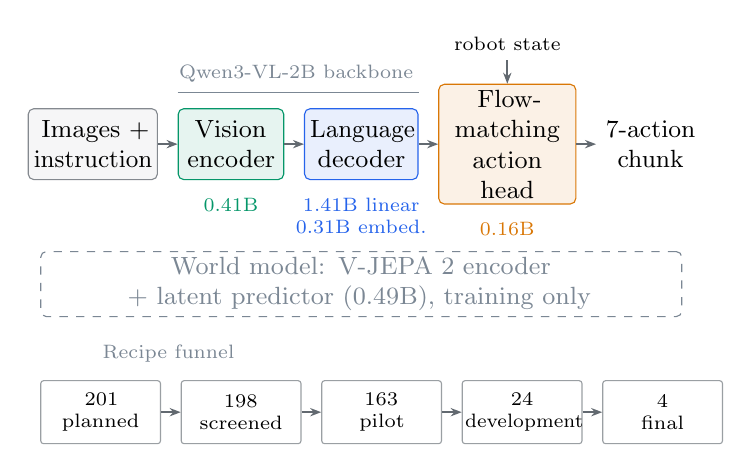
\begin{tikzpicture}[
  font=\small, node distance=3mm and 2.5mm,
  box/.style={draw=ink!55, rounded corners=2pt, fill=ink!4, align=center, minimum height=9mm, inner sep=2pt},
  tag/.style={font=\scriptsize, align=center},
  arr/.style={-{Stealth[length=4pt]}, draw=ink!70, line width=.6pt},
  funnel/.style={draw=ink!45, rounded corners=1pt, fill=white, align=center, font=\scriptsize, minimum height=8mm, inner sep=1pt, text width=14.5mm}]
\node[box, text width=15mm] (in) {Images +\\instruction};
\node[box, right=of in, text width=12mm, draw=vis, fill=vis!10] (vis) {Vision\\encoder};
\node[box, right=of vis, text width=13mm, draw=lang, fill=lang!10] (lm) {Language\\decoder};
\node[box, right=of lm, text width=16mm, draw=act, fill=act!10] (act) {Flow-matching\\action head};
\node[right=2.5mm of act, align=center] (out) {7-action\\chunk};
\draw[arr] (in) -- (vis); \draw[arr] (vis) -- (lm); \draw[arr] (lm) -- (act); \draw[arr] (act) -- (out);
\node[tag, below=1mm of vis, text=vis] {0.41B};
\node[tag, below=1mm of lm, text=lang] {1.41B linear\\0.31B embed.};
\node[tag, below=1mm of act, text=act] {0.16B};
\node[tag, above=3mm of act] (st) {robot state}; \draw[arr] (st) -- (act);
\draw[muted, line width=.5pt] ($(vis.north west)+(0,2mm)$) -- ($(lm.north east)+(0,2mm)$);
\node[tag, text=muted, above] at ($(vis.north)!0.5!(lm.north)+(0,2mm)$) {Qwen3-VL-2B backbone};
\node[box, dashed, fill=white, draw=muted, text=muted, minimum height=6mm,
  below=9mm of lm, text width=80mm]
  (wm) {World model: V-JEPA 2 encoder\\ + latent predictor (0.49B), training only};
\node[funnel, anchor=north west] (f1) at ($(wm.south west)+(0,-8mm)$) {201\\planned};
\node[funnel, right=2.5mm of f1] (f2) {198\\screened};
\node[funnel, right=2.5mm of f2] (f3) {163\\pilot};
\node[funnel, right=2.5mm of f3] (f4) {24\\development};
\node[funnel, right=2.5mm of f4] (f5) {4\\final};
\foreach \a/\b in {f1/f2,f2/f3,f3/f4,f4/f5} \draw[arr] (\a) -- (\b);
\node[tag, muted, above=1mm of f1, anchor=south west, xshift=-1mm] {Recipe funnel};
\end{tikzpicture}%
\caption{VLA-JEPA at inference, with parameter counts. Colored modules are the compression targets; the dashed world model is loaded but not run. Bottom strip: the recipe funnel. Three recipes failed the 80-frame screen at runtime, and the four final arms include the uncompressed control but not C2.}
\label{fig:arch}
\end{figure}

The uncompressed BF16 policy is called B16. Q4 quantizes every linear layer of the decoder to NF4, a 4-bit format with normal-float levels and double-quantized scales. Q8 does the same with LLM.int8. Every other module stays in BF16. The joint recipes quantize several modules at once. C1 keeps NF4 in the decoder and uses 2-bit HQQ in the vision and action modules. C2 uses NF4 everywhere and one flow step, with no pruning and no calibration data. Both joint recipes keep an 8-bit embedding table and drop the unused world model.

A sweep of 201 recipes applied quantizers (bitsandbytes INT8 and NF4, HQQ at 2 to 4 bits, GPTQ, AWQ-style scaling, TorchAO W8A8) and pruners (magnitude, Wanda and SparseGPT sparsity; structured removal of MLP channels, attention heads, layers and tokens) to single modules and combinations. Calibrated methods read frames from the development set only. Recipes that restrict the output vocabulary to this suite's instruction tokens are task-specific and stay out of Table~\ref{tab:results}, including two that reached held-out evaluation.

An automated coding agent proposed and screened recipes under one objective: the smallest configuration at 90\% success or better. Each had to pass a 10-trial pilot screen and score at least 77 of 100 on development; held-out trials were never used for selection. Q4 and Q8 are fixed comparison arms, and the joint recipes cleared the development gate before any held-out run.

Two targets: a 25\% cut in peak memory, the saving from 8-bit decoder weights alone (1.41\,GB of the 5.61\,GB peak, 25.1\%), and at most 5 success points lost against the uncompressed policy. Success carries 95\% Wilson intervals; differences use a paired bootstrap resampling within each task (10,000 resamples) over identical initial states and seeds, with gain/loss counts for episodes where only one arm succeeds.

LIBERO-Spatial is a simulated tabletop suite of ten pick-and-place tasks differing in object layout. Rollouts use all ten tasks, 50 initial states each, fixed per-episode seeds and a 280-step cap; an episode succeeds if the robot completes the instruction within the cap. Pilot, development and held-out use 10, 100 and 500 trials, development states disjoint from held-out. Latency is observation-to-action time, GPU-synchronized, over $3\times500$ predictions after 20 warm-up calls, simulator time excluded. Memory is peak allocated CUDA memory in GB ($10^9$ bytes). All held-out runs use one RTX 3090. The CUDA-graph engine precomputes instruction-dependent work, captures one graph per prompt, fuses elementwise operations with \texttt{torch.compile}, and dequantizes NF4 in one Triton kernel matching bitsandbytes bit for bit.

\section{Results}
Compression meets the memory and success targets on the decoder and joint recipes. Runtime execution, one sensitive task and a development-only search limit what each intervention achieves.

\subsection{Memory and latency}
Cutting peak memory from 5.61\,GB to 1.51\,GB requires compressing beyond the decoder, whereas cutting latency requires replacing PyTorch's stock (default) execution path, which is launch-bound (host-overhead-limited).

Q4 (decoder-only NF4) meets the memory target near the decoder-weight ceiling; Q8 (INT8) misses it, though both hold success inside the 5-point bound (Table~\ref{tab:results}, Fig.~\ref{fig:ladder}a). C1 and C2 both peak below 1.6\,GB. Only C2's paired gain has an interval clear of zero, and most of that gain comes from one task (Section~IV-C).

\begin{table}[t]
\centering\footnotesize\setlength{\tabcolsep}{2pt}
\caption{Held-out results: 500 rollouts per arm on an RTX 3090. Success is in percent, with a 95\% Wilson interval. $\Delta$ is the paired change from B16 in percentage points, with a task-stratified bootstrap interval. Gain/loss counts episodes where only that arm, or only B16, succeeds. Peak is allocated GPU memory, with the change from B16 in parentheses. C1 and C2 drop the unused world model; C2 runs on the graph engine with one flow step.}
\label{tab:results}
\begin{tabular}{@{}lcccc@{}}
\toprule
Arm & Success [95\% CI] & $\Delta$ [95\% CI] & Gain/loss & Peak GB (change) \\
\midrule
B16 & 95.0 [92.7, 96.6] & --- & --- & 5.61 \\
Q8 & 94.8 [92.5, 96.4] & $-0.2$ [$-1.2$, $+0.8$] & 3/4 & 4.30 ($-23$\%) \\
Q4 & 95.8 [93.7, 97.2] & $+0.8$ [$-0.6$, $+2.2$] & 8/4 & 3.54 ($-37$\%) \\
C1 & 96.8 [94.9, 98.0] & $+1.8$ [$-0.2$, $+3.8$] & 19/10 & 1.38 ($-75$\%) \\
C2 & 98.0 [96.4, 98.9] & $+3.0$ [$+1.4$, $+4.8$] & 18/3 & 1.51 ($-73$\%) \\
\bottomrule
\end{tabular}
\end{table}

On PyTorch's stock path every compressed model runs slower than its uncompressed control (Fig.~\ref{fig:ladder}b). The uncompressed policy was timed in two sessions; each comparison uses its own session's control. The INT8 decoder roughly doubles the median and the NF4 decoder adds 18\%, because the GPU idles while the CPU launches many small kernels.

\begin{figure*}[t]
\centering
\includegraphics{figures/ladder.pdf}
\caption{Peak memory (a) and median latency (b) along the path from the uncompressed policy to the joint recipes. (a) The dashed blue line is the NF4 ceiling for decoder weights, and the dashed grey line is the 25\% target at 4.20\,GB; bars that extend past it miss the target. (b) Dots mark medians and whiskers mark p95. The grey ticks are the two uncompressed controls, timed in separate sessions at 79.1 and 77.5\,ms. The arrow is the 6.8\,ms cost of packed over dense NF4 weights at one flow step.}
\label{fig:ladder}
\end{figure*}

The CUDA-graph engine removes most of that overhead for every variant (Fig.~\ref{fig:ladder}b, lower block). NF4 weights then cost time: at matched flow steps C2 takes 31.6\,ms against 24.8\,ms for the uncompressed policy on the same engine. Dense NF4 copies skip dequantization (unpacking weights before each product) but return peak memory to nearly the uncompressed level; packing keeps C2 small. C2's gain over the stock path therefore comes from the engine and the single flow step, which the pilot screen chose using outcomes but no held-out trial. On the stock path, lower memory did not reduce latency.

\subsection{Module sensitivity}
The language decoder sets the precision floor: pilot success holds near baseline at 7 of 10 for 3 and 4 bits and collapses to 1 of 10 at 2 bits, while vision and action modules keep full pilot success at 2 bits in their best tested variant (Fig.~\ref{fig:sens}a). Structured removal splits the same way: dropping 8 of 28 decoder layers or half its key--value heads collapses success, while vision tolerates losing half its channels or heads. Action modules lose success gradually.

The 10-trial screen is coarse and development has 100 trials: a 75\% cut of action attention heads passes the pilot at 7 of 10 yet fails the development gate of 77 (Fig.~\ref{fig:sens}d). On an NF4 base, combined channel cuts score 70 of 100 and combined depth cuts 65. Linear CKA (centered kernel alignment), the similarity of a block's output to its input, ranks depth cuts so the most redundant blocks go first. One decoder cut and one action cut each reached development at 80 of 100 [71.1, 86.7] and cleared the gate; neither entered a held-out arm.

\begin{figure*}[t]
\centering
\includegraphics{figures/sensitivity.pdf}
\caption{Module sensitivity from the 10-trial pilot screen. Each point is successes out of 10. The dotted line and shaded band are B16 at 8 of 10 with its 95\% interval, which is wide at this size. (a) Bit width for the language decoder, vision and action modules; the line joins the best variant at each width, and faint points are the other variants. (b--d) Share of each module removed. Missing points were not run because a milder cut had already failed. The callout in (d) gives development results, out of 100, for four cuts.}
\label{fig:sens}
\end{figure*}

\subsection{Failure concentration and offline screening}
One task drives most of the differences between arms: the uncompressed policy fails mostly in task 5, where it succeeds 33 times out of 50. Task 5 gives +11 of C1's net +9 episodes and +11 of C2's net +15; the other nine tasks give $-2$ for C1 and $+4$ for C2.

The gain follows the NF4 weights, not the engine or the flow-step count: the uncompressed policy on the engine scores 474 of 500, one episode below its stock-path result, while NF4 weights at four flow steps score 486 of 500, a paired gain of 2.2 points [+0.8, +3.8]. We do not know why task 5 responds this way, so we do not credit quantization with an improvement.

The offline measure works in one direction: it tracks pilot success across the sweep but not among the recipes that reached development (Fig.~\ref{fig:div}). It is the mean squared change in predicted arm commands against the uncompressed policy on fixed development frames, with no simulator. Near-lossless recipes still need closed-loop trials.

\begin{figure}[t]
\centering
\includegraphics{figures/divergence.pdf}
\caption{Each dot is one recipe. The horizontal axis is the mean squared change in predicted arm commands against the uncompressed policy on 80 fixed frames, on a log scale. The vertical axis is successes in the 10-trial pilot, jittered slightly. Dot color marks the module group changed, and dots at the far left have identical actions. Dashed guides at $10^{-4}$ and $10^{-3}$ divide the plot. Left of the first, nearly every recipe keeps 7 or more successes; right of the second, many do not.}
\label{fig:div}
\end{figure}

\subsection{Negative result: smaller backbone}
Replacing the Qwen backbone with SmolVLM2-500M and a trained adapter fails: 2.2\% success on 500 held-out trials (95\% interval 1.2 to 3.9), and about 16 times slower than the uncompressed policy. Adapting the four final decoder layers of the failed model reached 31 of 100 on development [22.8, 40.6] against 82 of 100 for B16 on the same states [73.3, 88.3]; no recovered model met the development gate. Within our budget, compression beats backbone replacement.

\subsection{Dream-RSI recipe search}
% DREAM-RSI: provisional, rewrite after new rounds
% reserved: one column-width figure (about 2.4 in) for the new rounds
Dream-RSI trims resident weights below the joint recipes, on development trials only. Its replay-picked search policy schedules 10-trial probes over hand-written grids, promoting the best to 100-trial development. Four restricted-vocabulary candidates scored 83 to 88 of 100 at 853 to 905\,MB resident (best: 88 of 100 [80.2, 93.0]). The 905\,MB point is Stage 2 (RTX 5060 Ti); the rest are replay-selected rounds on an RTX 3090. A full-vocabulary round reached 86 of 100 at 1,200\,MB. Two probes at 827 to 850\,MB failed the screen, a possible cliff on little data. Intervals overlap, nothing is held-out confirmed, and resident MB counts tensor bytes, not the peak memory of Table~\ref{tab:results}.

\section{Limitations and Conclusion}
These results cover LIBERO-Spatial, one checkpoint and one seed per state; the same 500 held-out states score every arm, with no correction for multiple comparisons. Other suites, real robots and other hardware were not measured. The graph engine assumes one observation, two equal-size images and unpadded prompts per call, and its fused kernels change BF16 rounding, so success was measured through the engine. Compressed archives are rebuilt from the checkpoint and a recipe, not standalone Hugging Face checkpoints.

Decoder-only NF4 meets the memory target with no detectable loss of success, and the joint recipes go further. The language decoder sets how far precision can fall. Compression alone made every model slower on the stock path, so speed depends on the execution engine as much as on the weights. Fused 4-bit kernels and longer-horizon suites are the next tests.

% AUTHORS: confirm contribution statement
\section*{Acknowledgment}
Noah Sprenger integrated the Dream-RSI engine and ran Stage 2; Fernando Nogueira ran the compression study and live Dream-RSI rounds; both authors wrote the report.

\bibliographystyle{IEEEtran}
\bibliography{refs}
\end{document}
